\documentclass[a4paper,11pt]{article}

\usepackage[utf8]{inputenc}
\usepackage[T1]{fontenc}
\usepackage[english]{babel}
\usepackage{graphicx}
\usepackage{amsmath,amssymb,amsthm,amsopn}
\usepackage{mathrsfs}
\usepackage{graphicx}
\usepackage{array}
\usepackage{makecell}


\usepackage{hyperref}
\hypersetup{
    colorlinks=true,
    linkcolor=blue,
    citecolor=red,
}

%\usepackage[top=1cm,bottom=1cm]{geometry}
%\usepackage{listings}
%\usepackage{xcolor}

\usepackage{tikz}

% Tikz style

\tikzset{round/.style={circle, draw=black, very thick, scale = 0.7}}
\tikzset{arrow/.style={->, >=latex}}
\tikzset{dashed-arrow/.style={->, >=latex, dashed}}

\input{thmstyle.tex}
% Math Operators

\DeclareMathOperator{\Card}{Card}
\DeclareMathOperator{\Gal}{Gal}
\DeclareMathOperator{\Id}{Id}
\DeclareMathOperator{\Img}{Im}
\DeclareMathOperator{\Ker}{Ker}
\DeclareMathOperator{\Minpoly}{Minpoly}
\DeclareMathOperator{\Mod}{mod}
\DeclareMathOperator{\Ord}{Ord}
\DeclareMathOperator{\ppcm}{ppcm}
\DeclareMathOperator{\Tr}{Tr}
\DeclareMathOperator{\Vect}{Vect}

% Shortcuts

\newcommand{\dE}{\partial(E)}
\newcommand{\dF}{\partial(F)}
\newcommand{\dG}{\partial(G)}
\newcommand{\diff}{\mathop{}\!\mathrm{d}}
\newcommand{\eg}{\emph{e.g. }}
\newcommand{\emb}{\hookrightarrow}
\newcommand{\embed}[2]{\phi_{#1\hookrightarrow#2}}
\newcommand{\ent}[2]{[\![#1,#2]\!]}
\newcommand{\ie}{\emph{i.e. }}
\newcommand{\ps}[2]{\left\langle#1,#2\right\rangle}
\newcommand{\eqdef}{\overset{\text{def}}{=}}


% opening
\title{Compatibility of embeddings using Allombert's algorithm}
\author{}



\begin{document}

\maketitle

%\begin{abstract}

%\end{abstract}

%\tableofcontents

%\clearpage

Assume we have three finite fields $K_1$, $K_2$, and $K_3$ such that
\[\partial(K_1)\,|\,\partial(K_2)\,|\,\partial(K_3),\]
and such that we already have $K_1\emb K_2$ and $K_1\emb K_3$, \ie such as in
Figure~\ref{fig:uncomplete}.
\begin{figure}
  \centering
    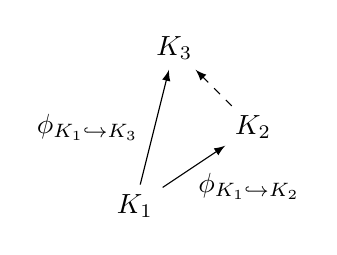
\begin{tikzpicture}
      \node (K1) at (0, 0) {$K_1$}; 
      \node (K2) at (1.5, 1) {$K_2$}; 
      \node (K3) at (0.5, 2) {$K_3$}; 

      \draw[arrow] (K1) -- (K2);
      \draw[arrow] (K1) -- (K3);
      \draw[dashed-arrow] (K2) -- (K3);

      \node (f12) at (1.45, 0.25) {$\embed{K_1}{K_2}$};
      \node (f13) at (-0.60, 1) {$\embed{K_1}{K_3}$};
    \end{tikzpicture}

  \caption{Uncomplete diagram of embeddings.}
  \label{fig:uncomplete}
\end{figure}
We are interested in the computation of the embedding $\embed{K_2}{K_3}$,
assuming we have computed the previous embeddings $\embed{K_1}{K_2}$ and
$\embed{K_1}{K_3}$ using Allombert's algorithm. We also assume that we have access
to the data used to compute these algorithms, such as the solutions of Hilbert
$90$ instances, or the roots involved.

\section{The easy case}

We first assume that $\partial(K_2)\,|\,p-1$, where $p$ is the caracteristic of
our finite fields. We denote $m=\partial(K_1)$ and $n=\partial(K_2)$, hence we
have $m$-th primitive roots of unity in $\mathbb{F}_p$ and $n$-th primitive
roots of unity also. Hence we are able to use Allombert's algorithm in the easy
case where we have enough roots in the base field. We denote by $\alpha_i$ the
solution of Hilbert $90$ solved in $K_i$, with some $m$-th primitive root of
unity $\zeta\in\mathbb{F}_p$ that was used for Allombert's algorithm. We also
note 
\[\embed{K_1}{K_2}:\alpha_1\mapsto c\alpha_2
\]
and
\[\embed{K_1}{K_3}:\alpha_1\mapsto d\alpha_3
\]
with $c, d\in\mathbb{F}_p$ the
elements computed during Allombert's algorithm.

Then, we compute a primitive $n$-th root of unity $\xi\in\mathbb{F}_p$ such that
\[
  \xi^{n/m}=\zeta.
\]
This is always possible since $\zeta$ is a $m$-th root of unity and $m|n$.
We solve (using linear algebra) Hilbert $90$ with the root
$\xi$ in $K_2$ and $K_3$ and denote by $\beta_2$ and $\beta_3$ the respective
nonzero solutions. We have
\[
  \sigma(\beta_i^{n/m})=\zeta\beta_i^{n/m}
\] for $i=2,3$. Since the solution of Hilbert $90$ is a one-dimensional
$\mathbb{F}_p$-vector space, we know that
\[
  \beta_i^{n/m}=a_i\alpha_i
\] for some $a_i\in\mathbb{F}_p^\times$. The compatibility condition imposes that 
\[
  \embed{K_1}{K_3}=\embed{K_2}{K_3}\circ\embed{K_1}{K_2},
\]
so we want to image of $\alpha_1$ in $K_2$ to be sent to $d\alpha_3$. In other
words, we want
\[
  \embed{K_2}{K_3}(c\alpha_2) = d\alpha_3.
\]
Hence, we want to find $e\in\mathbb{F}_p$ with $e^n=\beta_3^n/\beta_2^n$
and such that
\[
  e^{n/m}=a_2a_3^{-1}dc^{-1},
\]
since 
\[
  \alpha_2\mapsto c^{-1}d\alpha_3
\]
is the same as
\[
  a_2^{-1}\beta_2^{n/m}\mapsto c^{-1}da_3^{-1}\beta_3^{n/m}.
\]
By definition, we have that 
\begin{align*}
  (e^{n/m})^m &= \frac{(\beta_2^{n/m})^m}{(\beta_3^{n/m})^m}\\
  &= \left(\frac{a_2\alpha_2}{a_3\alpha_3}\right)^m\\
  &= \left(\frac{a_2\alpha_2\alpha_1}{a_3\alpha_1\alpha_3}\right)^m\\
  &= \left( a_2a_3^{-1}dc^{-1} \right)^m
\end{align*}
so $e^{n/m}$ might differ from $a_2a_3^{-1}dc^{-1}$ only by an $m$-th root of unity. Since $e$ is defined
up to multiplication by a $n$-th root of unity, we can find $e$ such that
$e^{n/m}=c^{-1}d$. With these choices of $\beta_2, \beta_3, e$ we have that 
\[
  \embed{K_2}{K_3}:\beta_2\mapsto e\beta_3
\]
is compatible with the already existing embeddings.
\end{document}
